\documentclass[aspectratio=169]{beamer}
\usetheme{Madrid}
\usecolortheme{beaver}
\usepackage[utf8]{inputenc}
\usepackage[T1]{fontenc}
\usepackage{tikz}
\usepackage{amssymb}
\usepackage{graphicx}
\setbeamertemplate{navigation symbols}{}
\setbeamercolor{title}{fg=white,bg=cyan!60!black}
\setbeamercolor{frametitle}{fg=white,bg=cyan!50!black}
\setbeamercolor{block title}{bg=cyan!15,fg=black}
\setbeamercolor{block body}{bg=cyan!5,fg=black}

\title{Block Arcade 2 — Motion \& Repeat}
\subtitle{Lesson 1: Repeat 3 Times}
\author{ByteForge --- Grade 7 --- Game Maker}
\date{}

\begin{document}

\begin{frame}
    \titlepage
\end{frame}

\begin{frame}{Repeat — do it without repeating yourself}
    \Large
    "Repeat 3" scales — drawing 30 sprites by hand would mean 30 blocks, while a repeat block handles any number.

    \begin{center}
    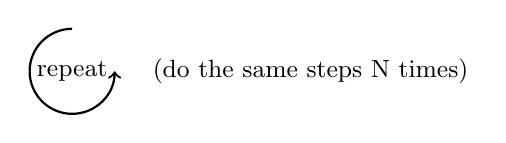
\begin{tikzpicture}[scale=0.9]

        \draw[->, thick] (0,0) arc (90:360:0.6);
        \node at (0,-0.6) {\small repeat};
        \node[right] at (1,-0.6) {\small (do the same steps N times)};
    \end{tikzpicture}
    \end{center}
\end{frame}

\begin{frame}{Your Turn}
    \Large
    Open the student map, find \textbf{Block Arcade 2 — Motion \& Repeat}, and complete
    the \textbf{Repeat 3 Times} challenge --- everything you just saw, they now do themselves.
\end{frame}

\end{document}
